\chapter{Basic Data Structures}


\section{Introduction}
Abstract Data Types (ADT):
\begin{enumerate}
\item Queue
\item Stack
\end{enumerate}
Implementation (for both queue and stack):
\begin{enumerate}
\item Linked List
\item Resizing Array:
\begin{enumerate}
\item Doubling: when full (100\%).
\item Halfing: when one-quarter full (100\%). 
\end{enumerate}}
\end{enumerate}}
Python Library:
\begin{enumerate}
\item \pythoninline{collections.deque} \footnote{The naming in collections is awkward: \href{http://stackoverflow.com/questions/18953681/naming-convention-in-collections-why-are-some-lowercase-and-others-capwords}{discussion}.}
\item \pythoninline{list}
\end{enumerate}} 
Java Library:
\begin{enumerate}
\item \javainline{java.util.Stack<E>}
\item \javainline{java.util.LinkedList<E>}
\end{enumerate}}

\section{Stack}
\subsection{Stack and Recursion}
How a compiler implements a function:
\begin{enumerate}
\item Function call: push local environment and return address
\item Return: pop return address and local environment. 
\end{enumerate}

Recursive function: function calls itself. It can always be implemented by using an explicit stack to remove recursion. 

\subsection{Largest Rectangle}
Find the largest rectangle in the matrix (histogram). Given $n$ non-negative integers representing the histogram's bar height where the width of each bar is 1, find the area of largest rectangle in the histogram. 

\begin{figure}[hbtp]
\centering
\subfloat{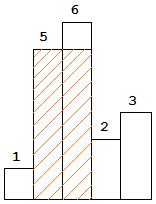
\includegraphics[scale=2.00]{histogram_area}}
\caption{Largest rectangle in histogram}
\label{fig:histogram_area}
\end{figure}

Keep a stack storing the bars in strictly increasing order, then calculate the area by popping out the stack to get the currently lowest bar which determines the height of the rectangle.

Notice:
\begin{enumerate}
\item Maintain the non-decreasing stack
\item Calculation of the rectangle width 
\item Post-processing in the end 
\end{enumerate}}
\begin{python}
def largestRectangleArea(self, height):
    n = len(height)
    gmax = -sys.maxint-1
    stk = []  # store the idx, non-decreasing stack

    for i in xrange(n):
        while stk and height[stk[-1]] > height[i]:
            last = stk.pop()
            if stk:  # calculate area when popping
                area = height[last]*(i-(stk[-1]+1))
            else:
                area = height[last]*i
            gmax = max(gmax, area)

        stk.append(i)

    # after processing all heights, process the remaining stack
    i = n
    ...

    return gmax
\end{python}

\section{Polish Notation}
Polish Notation is in-fix while Reverse Polish Notation is post-fix. 
\subsection{Evaluate Post-fix Expressions}
Straightforward: Use a stack to store the number. Iterate the input, push stack when hit numbers, pop stack when hit operators.
\subsection{Convert In-fix to Post-fix}


